\documentclass[./blockchain.tex
\graphicspath{{\subfix{./figures/}}}


\begin{document}

    \section{Web3-Anwendungen}

    \begin{frame}
        \frametitle{Was ist Web3}

        \begin{itemize}
            \item vereinfacht: Web3 ist die Technologie, mit welcher man mit dem Browser direkt mit einer Blockchain kommuniziert.
            \item Somit: Keine 'Backend', keine Datenbank, keine Passwort-Verwaltung, \ldots
        \end{itemize}

        \begin{center}
            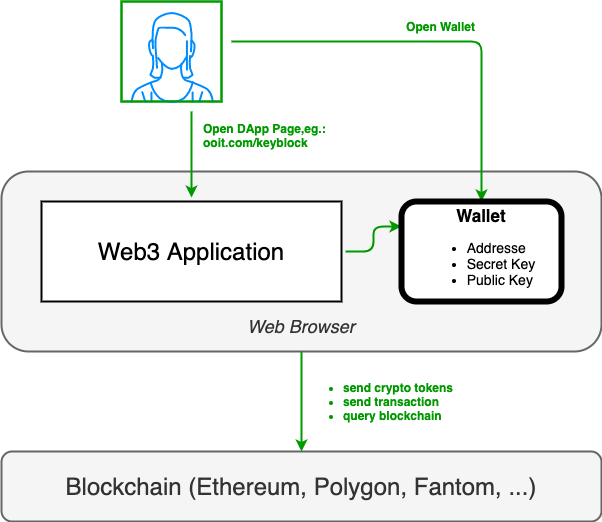
\includegraphics[width=0.40\textwidth]{figures/web3-architecture-Web3-simplified.drawio}
        \end{center}

    \end{frame}



    \begin{frame}
        \frametitle{Was ist Web3}{Voraussetzungen, Vorteile}

        \begin{itemize}
            \item Jede teilnehmende Person ist durch ihre Adresse identifiziert.
            \item Der Kommunikationspartner muss die Adresse kennen und sicher sein, welcher Person sie gehört.
            \item Die Adresse muss nicht geschützt werden. Sie sollte jedoch aus Datenschutzgründen vertraulich behandelt werden.
            \item Der Secret-Key verwaltet jeder Teilnehmer selber.
            \item Der Secret-Key wird technisch durch ein Wallet sicher verwaltet.
            \item Das Wallet kann allein die teilnehmende Person verwalten.
        \end{itemize}

    \end{frame}




    \begin{frame}
        \frametitle{Was ist Web3}{Weitere Eigenschaften}

        \begin{itemize}
            \item Mit dem Secret-Key können Meldungen und Transaktionen signiert werden.
            \item Mit dem Public-Key können Meldungen verschlüsselt übertragen werden.
            \item Bsp. Alice sendet eine Nachricht, welche mit ihrem Secret-Key signiert und mit dem Public-Key von Bob verschlüsselt wurde.
            \item \ldots Nur Bob kann die Nachricht mit seinem Secret-Key öffnen und mit dem Public-Key von Alice kann er die Signature überprüfen.
        \end{itemize}

    \end{frame}


    \begin{frame}{Web3 Anwendungen}{Globale D-Apps}
        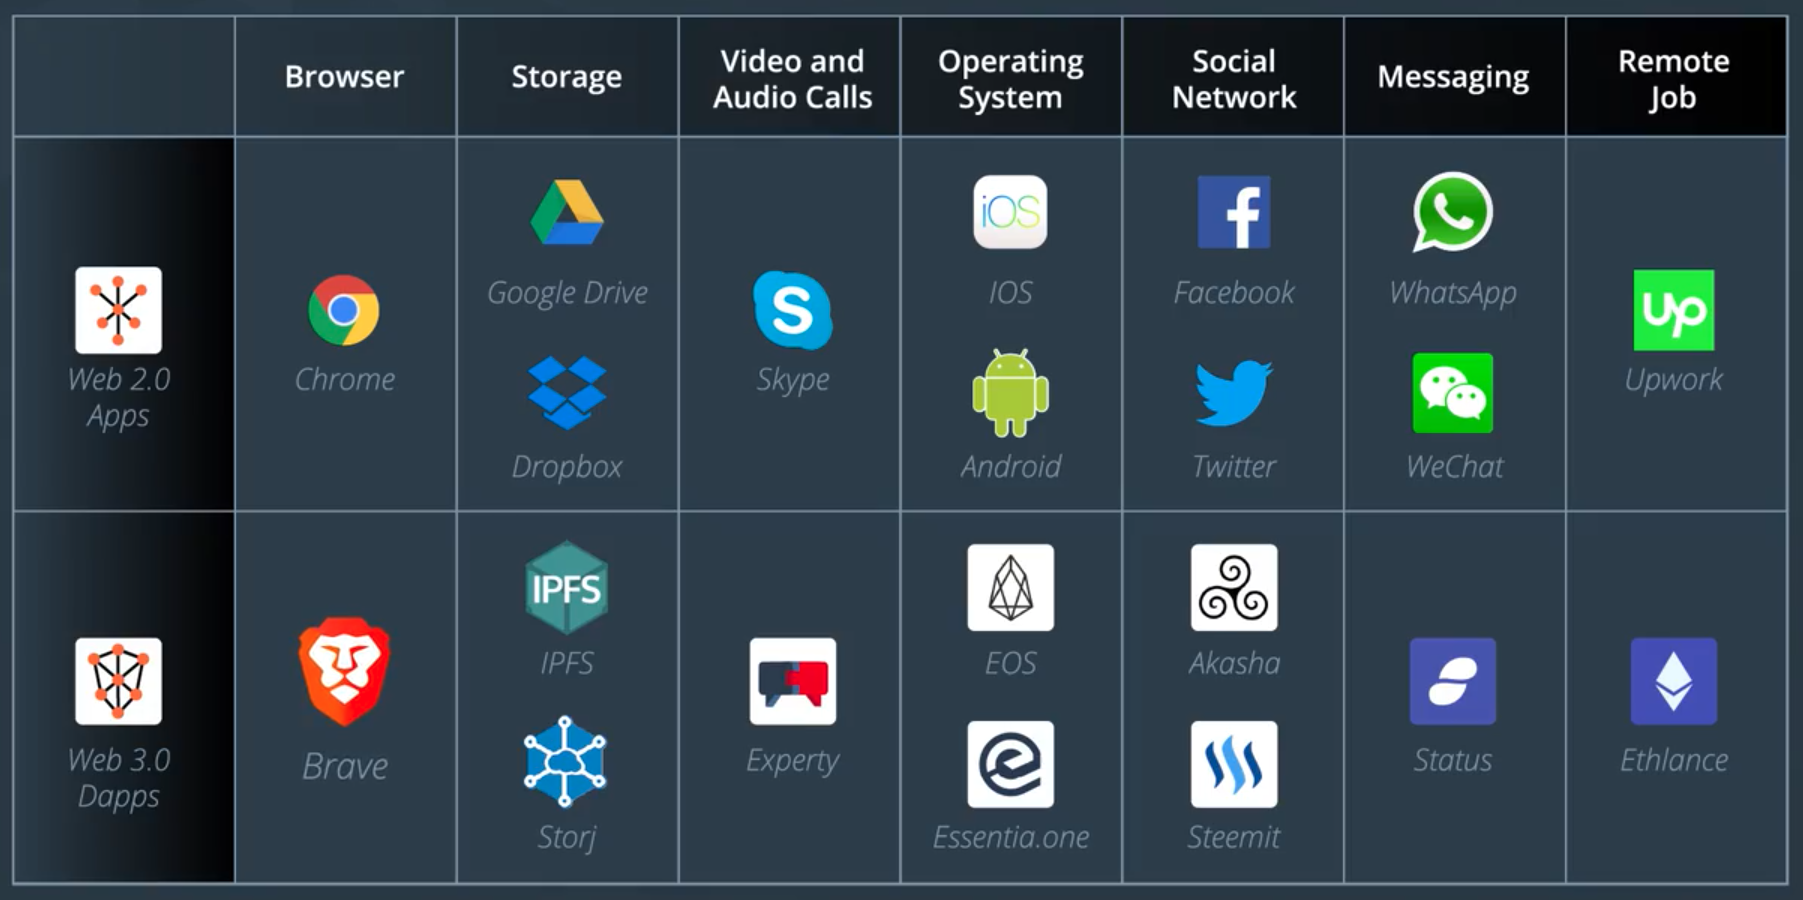
\includegraphics[width=0.99\textwidth]{figures/web3}
    \end{frame}


    \begin{frame}{Anwendungen}{Technischer Fokus}
        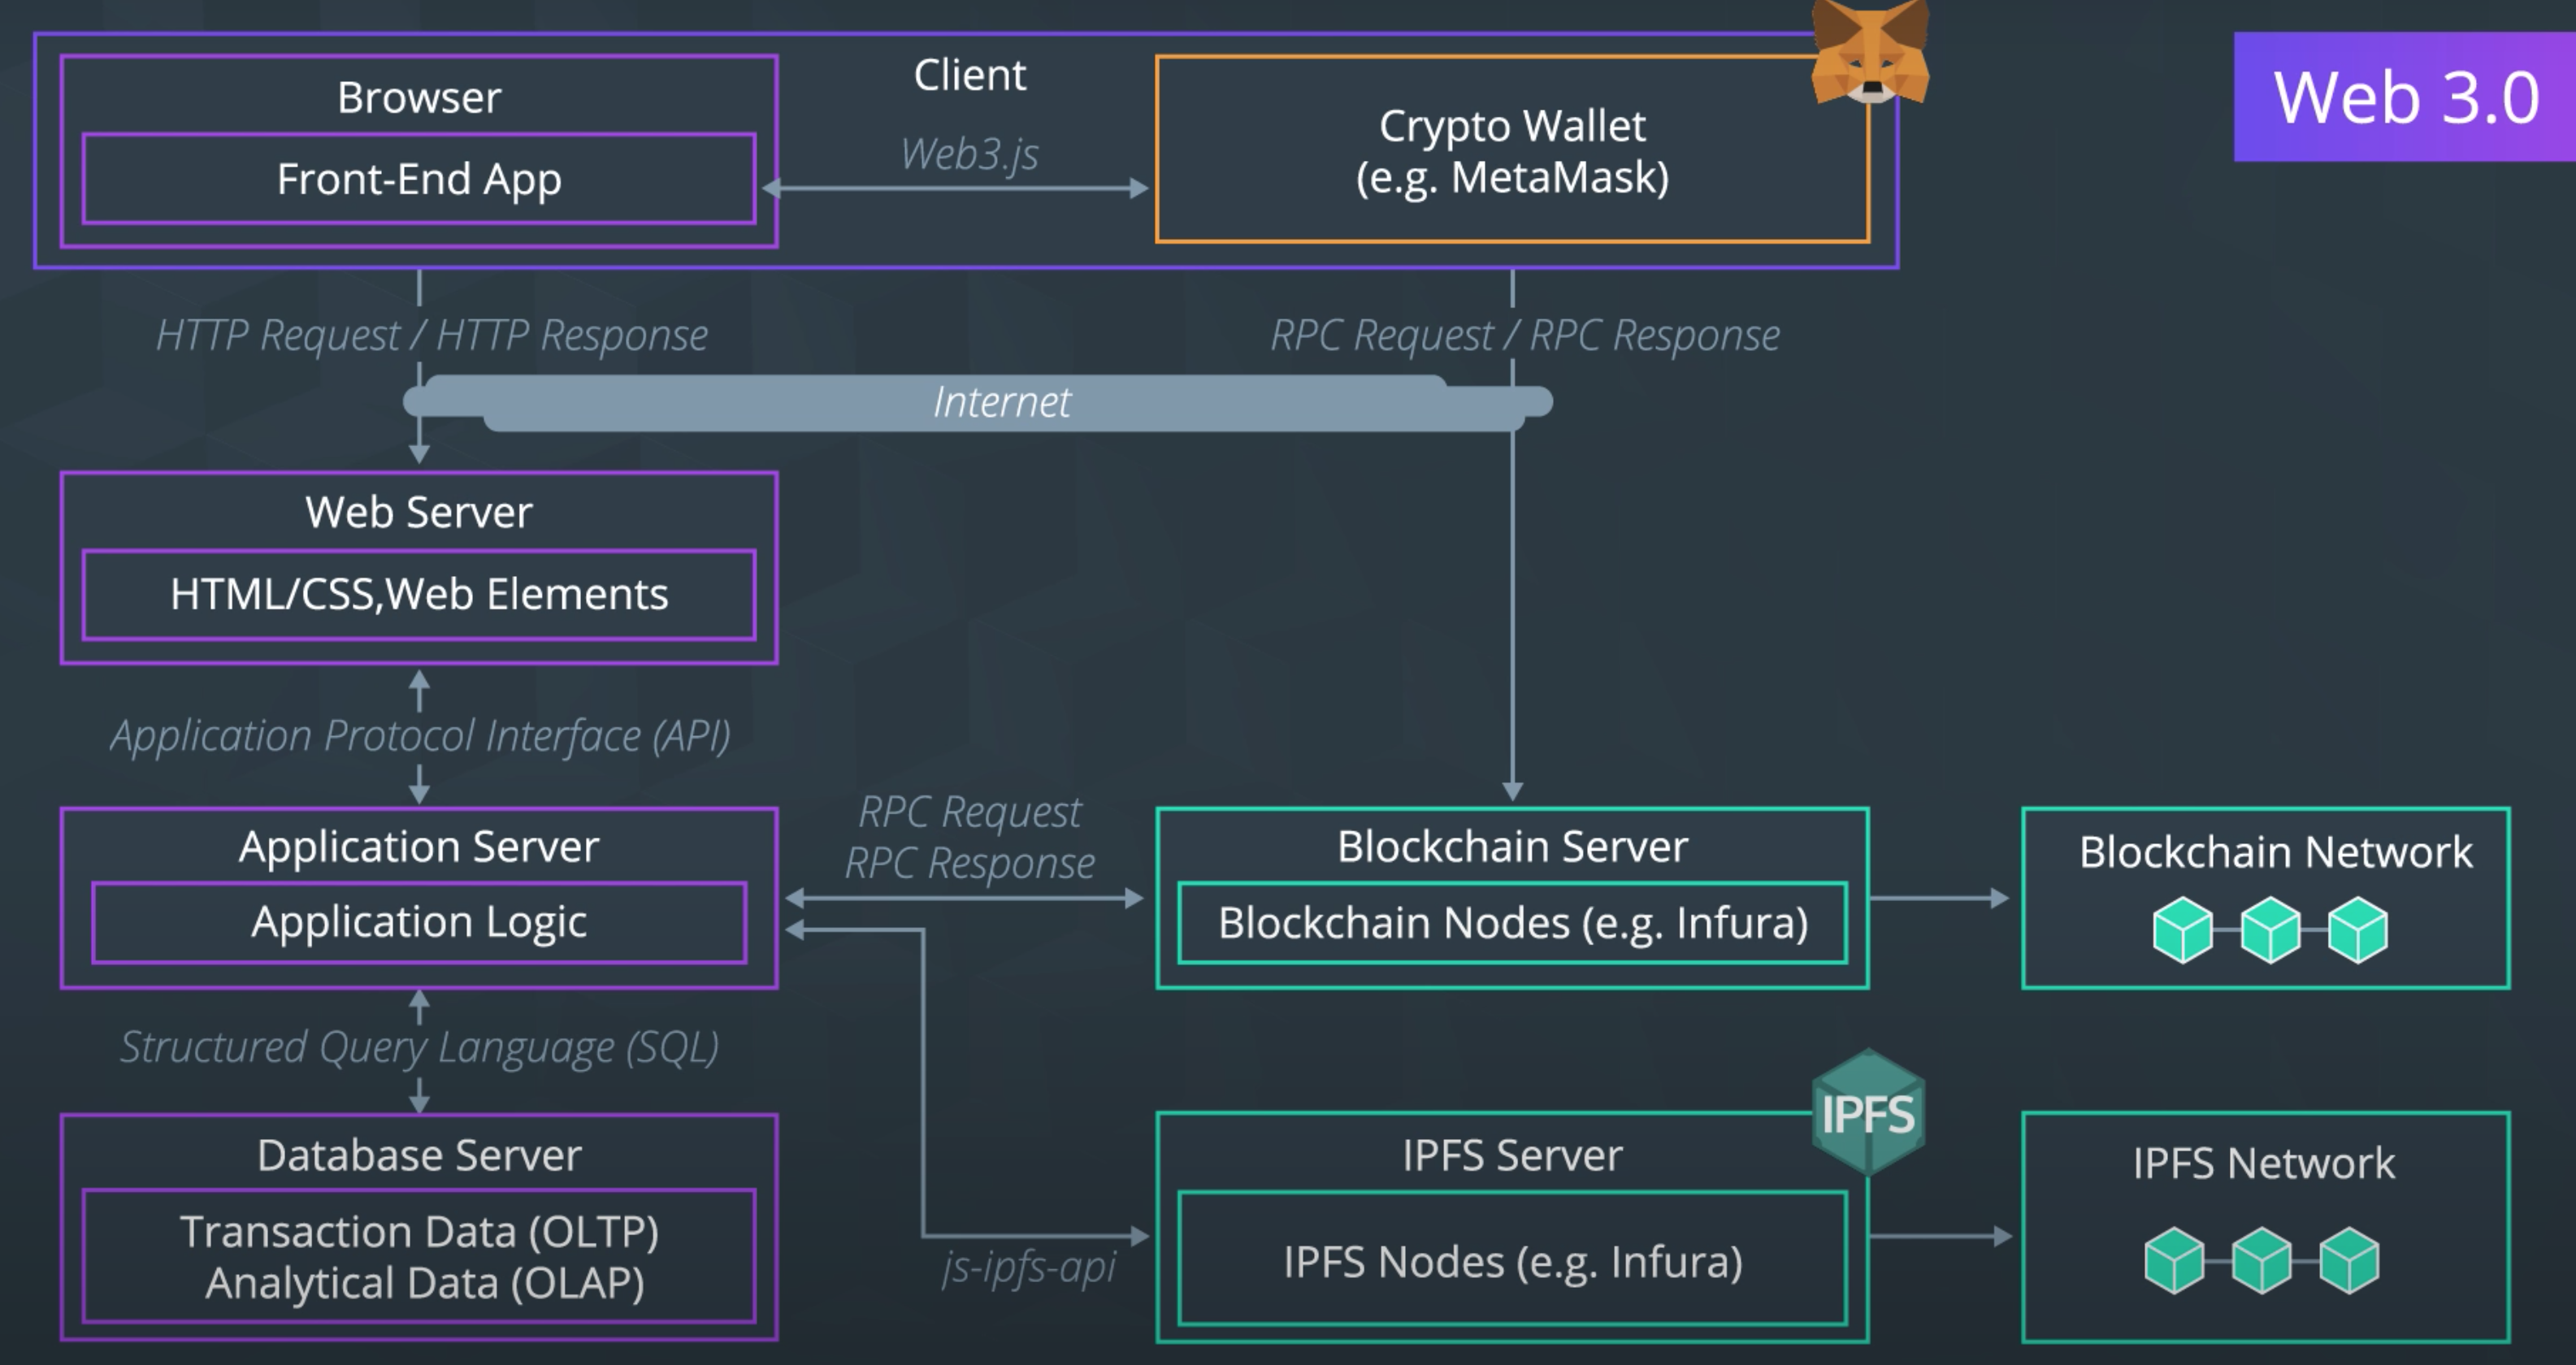
\includegraphics[width=0.99\textwidth]{figures/web3-interaction}
    \end{frame}


    \begin{frame}{Anwendungen für Individiual-Software}{User Login}
        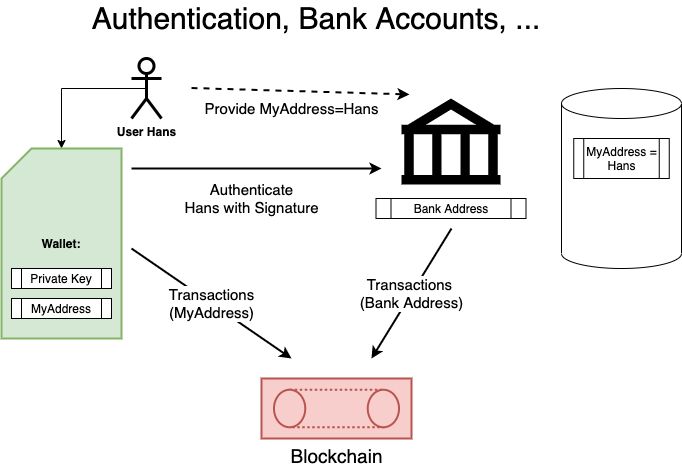
\includegraphics[width=0.80\textwidth]{figures/applications-user-login-with-blockchain.drawio}
    \end{frame}


    \begin{frame}{Anwendungsfall: Vertrauliche Nachrichten}{Ein zu eins Nachrichten}
    \end{frame}


\end{document}

